%% -*- coding: utf-8 -*-
\documentclass[12pt,a4paper]{scrartcl} 
\usepackage[utf8]{inputenc}
\usepackage[english,russian]{babel}
\usepackage{indentfirst}
\usepackage{misccorr}
\usepackage{graphicx}
\usepackage{amsmath}
\begin{document}
	\begin{titlepage}
		\begin{center}
			\large
			МИНИСТЕРСТВО НАУКИ И ВЫСШЕГО ОБРАЗОВАНИЯ РОССИЙСКОЙ ФЕДЕРАЦИИ
			
			Федеральное государственное бюджетное образовательное учреждение высшего образования
			
			\textbf{АДЫГЕЙСКИЙ ГОСУДАРСТВЕННЫЙ УНИВЕРСИТЕТ}
			\vspace{0.25cm}
			
			Инженерно-физический факультет
			
			Кафедра автоматизированных систем обработки информации и управления
			\vfill

			\vfill
			
			\textsc{Отчёт по практике}\\[5mm]
			
			\LARGE\textit{Вариант 7}
			
			{\LARGE Найти определитель матрицы}
			\bigskip
			
			1 курс, группа 1ИВТ АСОИУ
		\end{center}
		\vfill
		
		\newlength{\ML}
		\settowidth{\ML}{«\underline{\hspace{0.7cm}}» \underline{\hspace{2cm}}}
		\hfill\begin{minipage}{0.5\textwidth}
			Выполнил:\\
			\underline{\hspace{\ML}} К.\,В.~Рябенко\\
			«\underline{\hspace{0.7cm}}» \underline{\hspace{2cm}} 2024 г.
		\end{minipage}%
		\bigskip
		
		\hfill\begin{minipage}{0.5\textwidth}
			Руководитель:\\
			\underline{\hspace{\ML}} С.\,В.~Теплоухов\\
			«\underline{\hspace{0.7cm}}» \underline{\hspace{2cm}} 2024 г.
		\end{minipage}%
		
		
		\vfill
		
		
		
		\begin{center}
			
			Майкоп, 2024 г.
		\end{center}
	\end{titlepage}
\LARGE{Содержание}

\begin{enumerate}
	\item Задача
	\item Пример кода, решающего данную задачу
	\item Скриншот работы программы
\end{enumerate}
\section{Задача}
Найти определитель матрицы.
\section{Пример кода}
\label{sec:exp:code}
\begin{verbatim}
#include <iostream>

int determinant(int a1, int a2, int a3, int b1, int b2, int b3, int c1, int c2, int c3) {
    return a1 * (b2 * c3 - b3 * c2) -
           a2 * (b1 * c3 - b3 * c1) +
           a3 * (b1 * c2 - b2 * c1);
}

int main() {
    int a1 = 1, a2 = 0, a3 = -2;
    int b1 = -2, b2 = 4, b3 = 5;
    int c1 = 0, c2 = -3, c3 = 1;

    int det = determinant(a1, a2, a3, b1, b2, b3, c1, c2, c3);

    std::cout << "Определитель матрицы: " << det << std::endl;

    return 0;
}

	
	
	
\end{verbatim}
\vfill

\section{Скриншот работы программы}
\label{sec:picexample}
\begin{figure}[h]
	\centering
	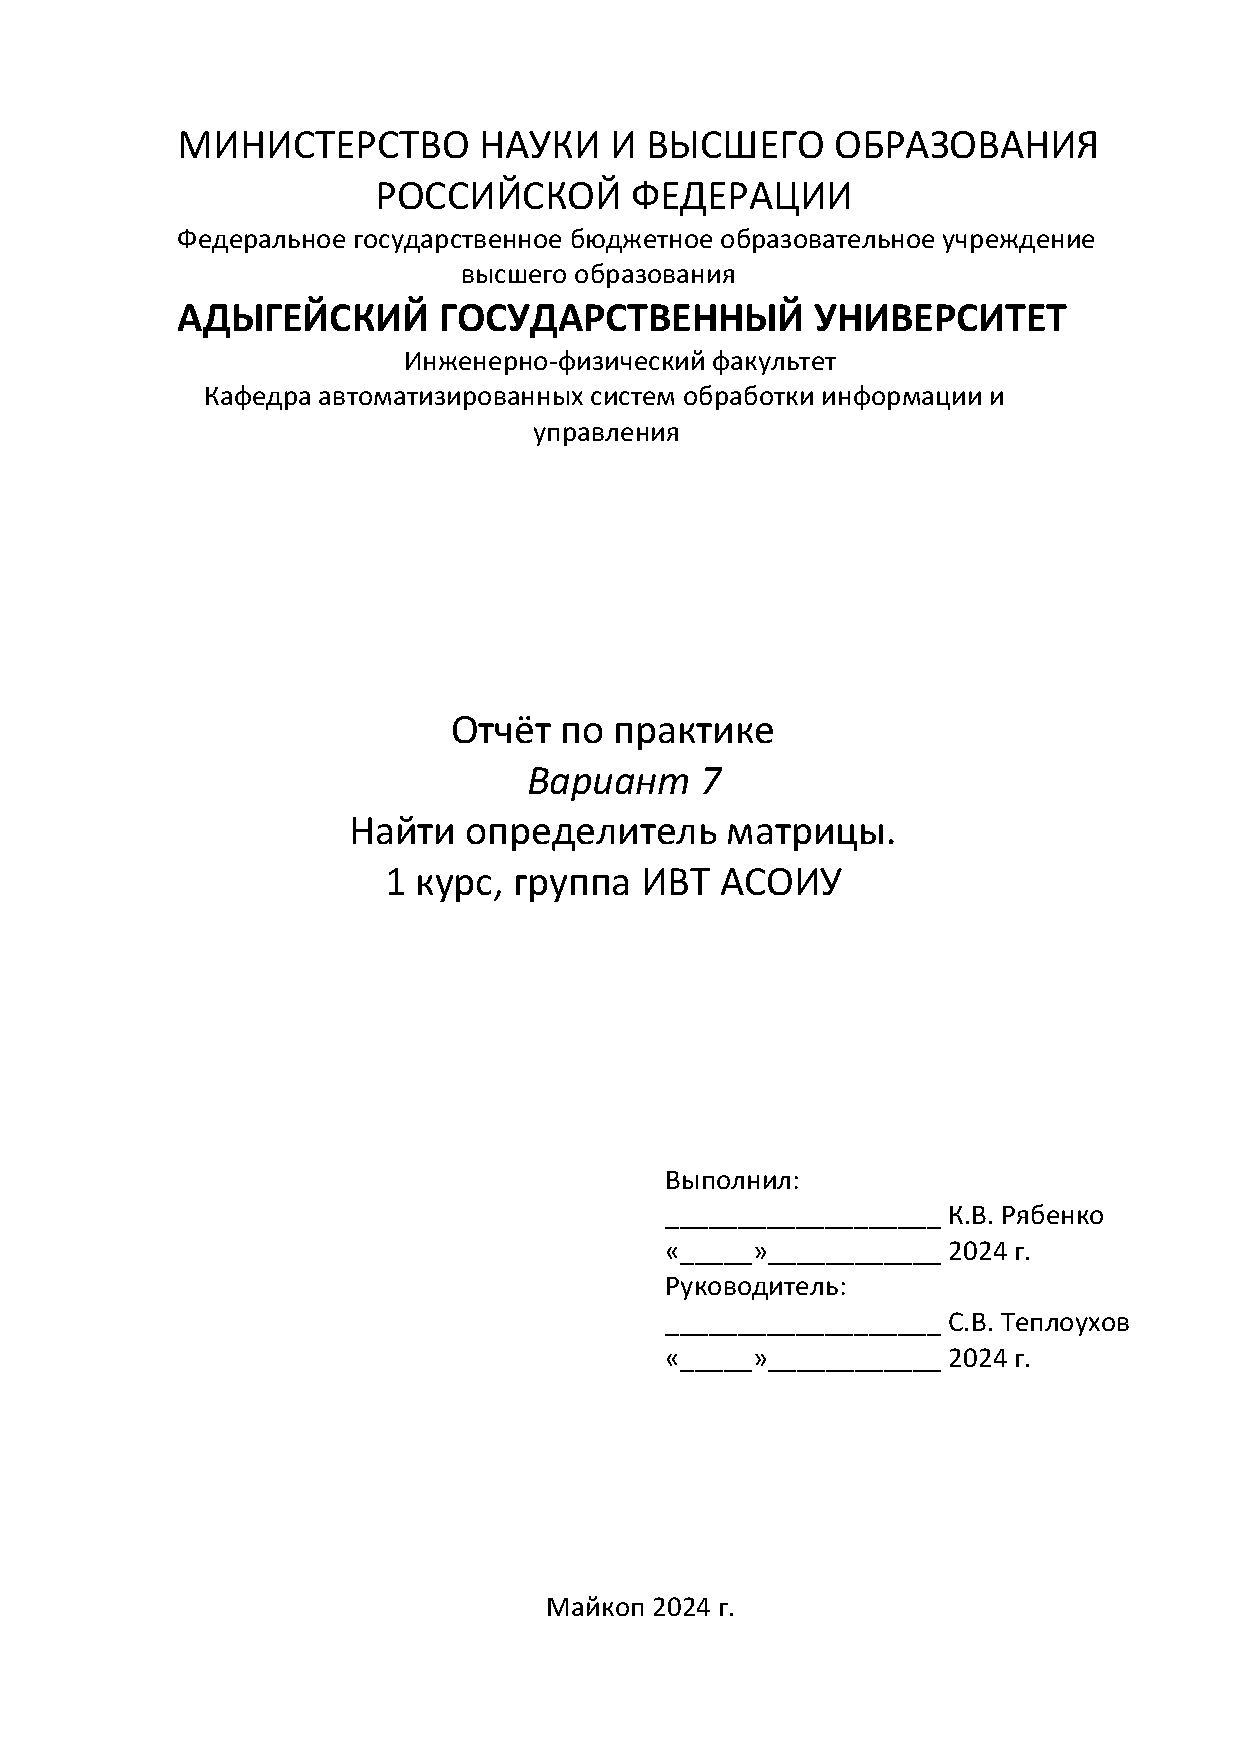
\includegraphics[width=0.9\textwidth]{Отчёт.png}
	\caption{Результат}\label{fig:par}
\end{figure}
\end{document}
